\begin{frame}{Conclusion: Model Performance}
By applying the test dataset on the model, the performance of the models can be evaluated. The accuracy summary of each 
model and the feature importance table from the best performing model is shown in \autoref{tab:acc_summary}.
\begin{table}
	\caption{Model Accuracy Summary}
	\centering
	\begin{tabular}{lrrr}
		\hline
		\textbf{Model} & \textbf{Accuracy} & \textbf{Micro-f1} & \textbf{Macro-f1} \\
		\hline
		Logistic Regression & 64.10\% & 0.6410 & 0.5863 \\
		Linear Perceptron & 48.72\% & 0.4872 & 0.2976 \\
		XGBoost & 76.92\% & 0.7692 &0.7749 \\
		\hline
	\label{tab:acc_summary}
	\end{tabular}
\end{table}
\end{frame}
\begin{frame}{Conclusion: Visualization}
Since XGBoost is the best performing model, its visualisation will be shown. 
\\The confusion matrix shows that most classes are classified correctly with the diagonal squares brighter than the others. However, due to the fact that level 4 has fewer data size than the others, it is hard to tell if it actually performs worse than the other levels. 

\begin{figure}[H]
    \centering
    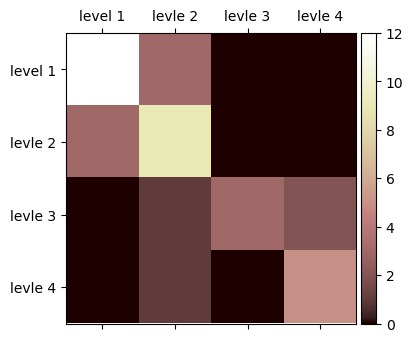
\includegraphics[width=0.4\linewidth]{images/illustrate/confma.jpeg}
    \caption{Confusion Matrix}
    \end{figure}

\end{frame}

\begin{frame}{Conclusion: Visualization}
In the normalised confusion matrix, it is clear that the darker square of level 4 is caused by the smaller data size of the class. The model is actually performing well even on smaller data size classes. That is why the macro-f1 is larger than micro-f1.

\begin{figure}[H]
    \centering
    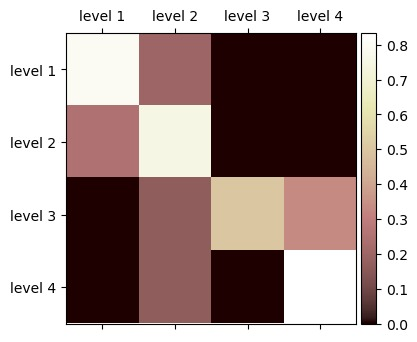
\includegraphics[width=0.5\linewidth]{images/illustrate/normconfma.jpeg}
    \caption{Normalized Confusion Matrix}
    \end{figure}
\end{frame}

\begin{frame} {Conclusion and Discussion}
From the feature importance table, it can be concluded that the severity of covid is more related 
to the human development index. The human development index is a score on the quality of living in the 
country including average life expectanvy, GDP, education opportunity, etc. The number of people fully 
vaccinated, the population composition or the diabetes prevalence do not play the most important role 
in the total cases as expected.   
\end{frame}